\section{Background: Goal-oriented Requirements Language and Argument Schemes}
\label{sect:background}

In this section, we first introduce and motivate the Goal-oriented Requirements Language (GRL), which is the goal modeling language used to connect to the argumentation framework. Next, we introduce and motivate \emph{the Argument Scheme for Practical Reasoning} (PRAS), which is a particular argument scheme that is used to form arguments and counter-arguments about situations involving goals.

\subsection{Goal-oriented Requirements Language (GRL)}
\label{sect:background:grl}
GRL is a visual modeling language for specifying intentions, business goals, and non-functional requirements (NFRs) of multiple stakeholders \cite{Amyot:2010:EGM:1841349.1841356}. It can be used to specify alternatives that have to be considered, decisions that have been made, and rationales for making decisions. A GRL model is a connected graph of intentional elements that optionally are part of actors. Figure~\ref{fig:trafficsim} illustrates a GRL diagram. An actor (
\includegraphics[scale=1]{img/actor}) represents a stakeholder of a system (\textbf{User}, Figure~\ref{fig:trafficsim}), or the system itself (\textbf{Simulation}, Figure~\ref{fig:trafficsim}). Actors are holders of intentions; they are the active entities in the system or its environment who want goals to be achieved, tasks to be performed, resources to be available, and softgoals to be satisfied. Softgoals (
\includegraphics[scale=1]{img/softgoal}) differentiate themselves from goals (
\includegraphics[scale=1]{img/goal}) in that there is no clear, objective measure of satisfaction for a softgoal whereas a goal is quantifiable, often in a binary way. Softgoals (e.g. \textbf{Realistic simulation)} are often more related to NFRs, whereas goals (such as \textbf{Generate traffic}) are more related to functional requirements. Tasks (
\includegraphics[scale=1]{img/task}) represent solutions to (or operationalizations of) goals and softgoals. In Figure~\ref{fig:trafficsim}, some of the tasks are \textbf{Create new cars} and \textbf{Keep same cars}. In order to be achieved or completed, softgoals, goals, and tasks may require resources (
\includegraphics[scale=1]{img/resource}) to be available (e.g. \textbf{******})

\begin{figure*}[ht]
\centering
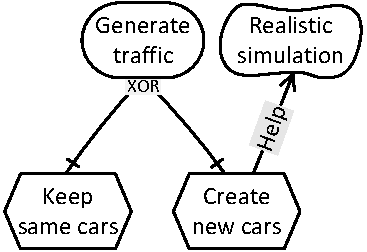
\includegraphics[]{img/Example}
\caption{GRL Model for the traffic simulator}
\label{fig:trafficsim}
\end{figure*}

Different links connect the elements in a GRL model. AND, IOR, and XOR decomposition links (
\includegraphics[scale=1]{img/decomposition}) allow an element to be decomposed into sub-elements. In Figure~\ref{fig:trafficsim}, the goal \textbf{Generate traffic} is XOR-decomposed to the tasks \textbf{Create new cars} and \textbf{Keep same cars}. Contribution links (
\includegraphics[scale=1]{img/contribution}) indicate desired impacts of one element on another element. A contribution link has a qualitative contribution type or a quantitative contribution. Task \textbf{Create new cars} has a \textbf{help} qualitative contribution to the softgoal \textbf{Realistic simulation}. Dependency links (
\includegraphics[scale=1]{img/dependency}) model relationships between actors. For example, actor \textbf{Simulation} depends on the actor \textbf{User} to perform the task \textbf{Adjust car spawning rate} to fulfil its task \textbf{Create new cars}.

GRL is based on $i*$~\cite{Yu:1997:TMR:827255.827807} and the NFR Framework~\cite{chung2012non}, but it is not as restrictive as $i*$. Intentional elements and links can be more freely combined, the notion of agents is replaced with the more general notion of actors, i.e., stakeholders, and a task does not necessarily have to be an activity performed by an actor, but may also describe properties of a solution. GRL has a well-defined syntax and semantics, which are necessary if we want to incorporate it into a formal framework (requirements 1 and 2 as described in the introduction). Furthermore,GRL provides support for providing a scalable and consistent representation of multiple views/diagrams of the same goal model (see~\cite[Ch.2]{Ghanavati2013} for an more details). For example, traceability links are provided between between concepts and instances of goal modeling and behavioral design models \cite{}. Multiple views and traceability are a good fit with our current research: we aim to add traceability links between intentional elements and their underlying arguments. \todo{Sepideh}{Sepideh}{I need to improve: GRL has has the capability to be extended via profile, metadata and rules, and due to this capability, it has been extended to many domain. This feature also helps us to apply our argumentation to other domain such as compliance or enterprise architecture. }

\subsubsection{Traffic simulator example}
\label{sect:background:casestudy}

In this paper, we use for our examples materials from our case study on the architecture for a traffic simulator \cite{}. \todo{Floris}{all}{briefly explain the traffic simulation case and the GRL model}

The GRL model in Figure~\ref{fig:trafficsim} shows the softgoals, goals, tasks and the relationship between the different intentional elements in the model. However, the rationales and arguments behind certain intentional elements have not been discussed or illustrated in the GRL model. Some of the questions that might be interesting to know about are the following:

\todo{Floris}{all}{These have to be amended}
\begin{itemize}
	\item Why are only the two softgoals \textbf{Quick} and \textbf{Low effort} selected for the task \textbf{Organize Meeting}? Why is, for example, a goal \textbf{Selecting the most convenient time} not included in the analysis for the actor \textbf{Meeting Initiator}?
	\item What does \textbf{Quality of Proposed Date} mean?
	\item How can one decide if the quality is low or high? Who is in charge? \todo{Floris}{Sepideh}{do you mean the \textbf{Quality of Proposed Date}? Or quality of the GRL diagram?}
	\item Does the meeting initiator use an email to inform the meeting participants to enter their availabilities? 
	\item Does the meeting scheduler uses an online calendar to obtain the available dates or an online website?
	\item How much time do the participants have to enter their availabilities? Is that important? Do they get a reminder from either the initiator or the scheduler? Is the reminder sent via an email? 
	\item What does \textbf{Richer Medium} mean? 
\end{itemize}

These are the type of the questions that we cannot answer just by looking at the GRL models. The model in figure~\ref{fig:trafficsim} does not contain information about discussions that let up to the resulting elements of the model, such as by various clarification steps for the naming, or alternatives that have been considered for the relationships. In order to address this, we use Argument Schemes for Goal Modeling (GMAS). GMAS can help us decide what intentional elements should remain in GRL and what new ones to be added or deleted, provide rationale behind the design decisions and the relationships between the links. 

\subsection{Argument Scheme for Practical Reasoning (PRAS)}
\label{sect:background:pras}

Reasoning about which goals to pursue and actions to take is often referred to as \emph{practical reasoning}, and has been studied extensively in philosophy (e.g. \cite{Raz1978-RAZPR,walton1990}) and Artificial Intelligence \cite{Bratman1987,atkinson2007}. One approach is to capture practical reasoning in terms of arguments schemes and critical questions~\cite{walton1990}. The idea is that an instantiation of such a scheme gives a presumptive argument in favor of, for example, taking an action. This argument can then be tested by posing critical questions about, for instance, whether the action is possible given the situation, and a negative answer to such a question leads to a counterargument to the original presumptive argument for the action. 

A formal approach to persuasive and deliberative reasoning about goals and actions has been presented by Atkinson et al.~\cite{atkinson2007}, who define the Practical Reasoning Argument Scheme (PRAS). PRAS follows the following basic argument structure. 

\begin{itemize}
\item[] We have goal $G$,
\item[] Doing action $A$ will realize goal $G$,
\item[] Which will promote the value $V$
\item[] \textit{Therefore} 
\item[] We should perform action $A$
\end{itemize}

So, for example, we can say that 
\begin{itemize}
\item[] We have goal \textbf{Generate traffic},
\item[] \textbf{Keep same cars} will realize goal \textbf{Generate traffic},
\item[] Which will promote the value \textbf{Simple design}
\item[] \textit{Therefore} 
\item[] We should perform action \textbf{Keep same cars}
\end{itemize}

Practical reasoning is defeasible, in that conclusions which are at one point acceptable can later be rejected because of new information. Atkinson \emph{et al.}~\cite{atkinson2007} define a set of critical questions that point to typical ways in which a practical argument can be criticized by, for example, questioning the validity of the elements in the scheme or the connections between the elements. Some examples of critical questions are as follows.

\begin{enumerate}
\item Will the action bring about the desired goal?
%\item Does the goal promote the value stated?
\item Are there alternative ways of realizing the same goal?
\item Are there alternative ways of promoting the same value?
%\item Does doing the action have a side effect which demotes the value?
\item Does doing the action have a side effect which demotes some other value?
\item Does doing the action promote some other value?
%\item Does doing the action preclude some other action which would promote some other value?
\item Is the action possible?
\item Can the desired goal be realized?
\item Is the value indeed a legitimate value?
\end{enumerate}

These critical questions can point to new arguments that might counter the original argument. Take, for example, critical question 4: if we find that \textbf{Keep same cars} actually negatively influences the value \textbf{Realistic simulation}, we have a counterargument to the above argument. Another way to counter an argument for an action is to suggest an alternative action that realizes the same goal (question 2) or an alternative goal that promotes the same value (question 3). For example, we can argue that \textbf{Create new cars} also realizes the goal \textbf{Generate traffic}, which gives us a counterargument to the original argument -- to generate traffic by simply keeping the cars that disappear off the screen and have them wrap around to the other side of the screen -- that also follows PRAS. 

In argumentation, counterarguments are said to \emph{attack} the original arguments (and sometimes vice versa). In the work of Atkinson et al.~\cite{atkinson2007}, arguments and their attacks are captured as an \emph{argumentation framework} of arguments and attack relations as introduced by Dung~\cite{Dung1995}\footnote{Full definitions of Dung's~\cite{Dung1995} frameworks and semantics will be given in section \ref{sect:gmas}. In this section, we will briefly discuss the intuitions behind these semantics.}. Figure \ref{fig:pras:example1} shows an argumentation framework with three arguments from the above example: the argument for \textbf{Keep same cars} (A1), the argument for \textbf{Create new cars} (A3), and the argument that \textbf{Keep same cars} demotes the value \textbf{Realistic simulation} (A2). The two alternative PRAS instantiations are A1 and A3. These arguments mutually attack each other, as \textbf{Keep same cars}  and \textbf{Create new cars} are considered to be mutually exclusive. Argument A2 attacks A1, as it points to a negative side-effect of \textbf{Keep same cars}. 

\begin{figure}[ht]
\centering
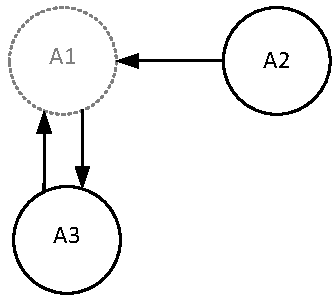
\includegraphics[scale=0.8]{img/Fig1}
\caption{Argumentation framework}
\label{fig:pras:example}
\end{figure}

Given an argumentation framework, the acceptability of arguments can be determined according to the appropriate argumentation semantics. The intuition is that an argument is acceptable if it is \emph{undefeated}, that is, any argument that attacks it, is itself defeated. In the argumentation framework in Figure~\ref{fig:pras:example}, argument A2 is undefeated because it has no attackers. This makes A1 defeated, because one of its attackers, A2, is undefeated. A3 is then also undefeated, since its only attacker, A1, is defeated by A2. Thus, the set of undefeated (justified) arguments given the argumentation framework in Figure~\ref{fig:pras:example} is $\{$A2, A3$\}$. 

In some cases, it is more difficult to determine whether or not an argument is defeated. Take, for example, the argumentation framework with just A1 and A3: they attack each other, they are alternatives and without any explicit preference, it is impossible to choose between the two. It is, however, possible to include explicit preferences between arguments when determining argument acceptability \cite{amgoud2002reasoning}. Take, for example, A1 and A3. If we say that we prefer the action \textbf{Create new cars} (A3) over the action \textbf{Keep same cars} (A1), we remove the attack from A1 to A3 (Figure~\ref{fig:pras:example2}, left). This makes A3 the only undefeated argument, whereas A1 is now defeated. It is also possible to give explicit arguments for preferences \cite{modgil2009}. These arguments are then essentially attacks on attacks. For example, say we prefer A3 over A1 because `it is important to have realistic traffic flows' (A4). This can be rendered as a separate argument that attacks the attack from A1 to A3 (Figure~\ref{fig:pras:example2}, right), removing this attack and making $\{$A3, A4$\}$ the undefeated set of arguments.

\begin{figure}[ht]
\centering
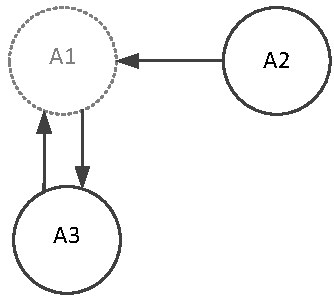
\includegraphics[scale=0.8]{img/Fig2}
\caption{Preferences between arguments}
\label{fig:pras:example2}
\end{figure}  

\subsubsection{Practical Argumentation and Goal Modeling}
\label{sect:background:pras:motivation}

Practical reasoning in the PRAS framework as described above provides a formally sound framework for defeasible reasoning about goals and actions that adheres to the acceptability semantics of Dung~\cite{Dung1995} and its various extensions \cite{amgoud2002reasoning,modgil2009}. The usefulness of PRAS for the analysis of practical reasoning situations has been shown in different areas such as e-democracy~\cite{cartwright2009IS}, law~\cite{atkinson2005legal}, planning \cite{medellin2013planning} and choosing between safety critical actions \cite{tolchinsky2012deliberation}. The question in this paper is how PRAS can be adopted for use in goal modeling, so that we can capture the discussions between stakeholders that build a goal model as formal argumentation, thus adding a new evaluation technique for goal models that allows us to assess the \emph{acceptability} of elements of a goal model (as opposed to the \emph{satisfiability} \cite{Amyot:2010:EGM:1841349.1841356}).

As can be seen in the above examples, PRAS (actions, goals, values) and GRL (tasks, goals, softgoals) have some obvious similarities. One way to connect goal modelling and argumentation is to build practical reasoning arguments based on PRAS and then translate these to goal models, or vice versa (Figure~\ref{fig:pras:example3}). This is essentially what happens in much of the existing work on argumentation and goal modelling \cite{Jureta:RE2008,vanzee-etal:renext2015,vanZee-etal:er2016} 

\begin{figure}[ht]
\centering
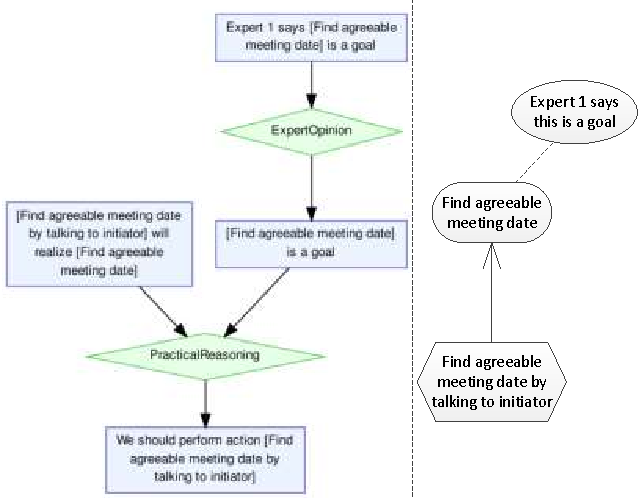
\includegraphics[width=\columnwidth]{img/Fig3}
\caption{Translating between practical reasoning argument (left) and GRL diagram (right)}
\label{fig:pras:example3}
\end{figure}  

One question is what the added value is of the direct translations as shown in Figure~\ref{fig:pras:example3}. The idea is that arguments show the rationales behind goal models and the alternative or possibly conflicting views that were lost in the goal-modeling process. However, GRL already contains a \emph{belief} element that allow one to provide beliefs underlying a goal model, an \emph{XOR decomposition} link that allows for modeling of alternative ways to realize goals, and \emph{negative contribution} links for capturing conflicting goals. So argumentation models are not needed to precisely render goals, tasks, beliefs and the relations between them, as GRL is already perfectly suited for this. Rather, argumentation should guide the goal modelling \emph{process}. 

In order for an argumentation-based framework to captures discussions about goal models, it should capture the dynamic, question-answer interplay between argument and counterargument. Argumentation schemes and their associated critical questions are ideally suited for this: as Murukannaiah et al.~\cite{murukannaiah2015} have shown, argumentation schemes and critical questions can guide users in systematically deriving conclusions and making their assumptions explicit. Furthermore, if we want to allow for the (semi-)automated construction of goal models given arguments and counterarguments, the argumentation framework needs to have a proper dialectical semantics \cite{Dung1995}. This means that the basic ideas of Atkinson et al.'s~\cite{atkinson2007} practical reasoning -- goal-based arguments and critical questions combined with the acceptability semantics of Dung -- can be used in our RationalGRL framework, as will be discussed in section \ref{sect:gmas}.
